\hypertarget{header}{}
\hypertarget{mini-projet-web}{%
\section{Mini projet WEB}\label{mini-projet-web}}

\includegraphics[width=1.66667in,height=\textheight]{img/html.png}

\hypertarget{content}{}
\hypertarget{introduction}{%
\subsection{Introduction}\label{introduction}}

Ce mini projet a pour objectif de créer un site WEB constitué de trois
pages écrites en langages HTML, CSS et JAVASCRIPT. Le sujet traité par
le site est libre mais doit être relatif à la vie lycéenne comme une
sortie scolaire, un enseignement suivi, la présentation d'un club, les
activités sportives ou artistiques au lycée, etc.

Les trois pages du site WEB se répartissent ainsi:

\begin{enumerate}
\tightlist
\item
  La première page est l'accueil du site;
\item
  La seconde page est une exposition de photographies;
\item
  La dernière page contient un formulaire de contact.
\end{enumerate}

\hypertarget{la-charte-technique-du-site}{%
\subsection{La charte technique du
site}\label{la-charte-technique-du-site}}

Les fichiers du site sont rassemblés dans un même dossier nommé
\textbf{projet}. \includegraphics{img/arbo_projet.png}

\begin{enumerate}
\tightlist
\item
  Le dossier \textbf{projet} contient les dossiers \textbf{css},
  \textbf{js} et \textbf{img} ainsi que les trois fichiers HTML
  \textbf{accueil.html}, \textbf{contact.html} et
  \textbf{diaporama.html}.
\item
  Le dossier \textbf{css} contient la feuille de style
  \textbf{style.css}.
\item
  Le dossier \textbf{js} contient les 2 fichiers javascript
  \textbf{slide.js} et \textbf{formulaire.js}.
\item
  Le dossier \textbf{img} contient toutes les photos et images du site
  WEB.
\end{enumerate}

\hypertarget{les-fichiers-html}{%
\subsection{Les fichiers HTML}\label{les-fichiers-html}}

Les fichiers HTML ont la même structure appelée \textbf{squelette}
utilisé pour toute page HTML avec les balises html, head, title, body,
etc. Le contenu placé entre les balises \textless body\textgreater{} et
\textless/body\textgreater{} est divisé en trois blocs délimités par les
balises html \textless div\textgreater{} et \textless/div\textgreater.

Un modèle de page web est donné pour la mise en place de ces trois
blocs. Il sera à adapter pour chacune de vos pages.

\includegraphics{img/squelette_page.png}

\begin{enumerate}
\tightlist
\item
  Le premier bloc contient le titre du site WEB présent sur les trois
  pages WEB.
\item
  Le second bloc est dédié au contenu différent pour chaque page du
  site.
\item
  Le dernier bloc est un pied de page que l'on retrouve sur les trois
  pages.
\end{enumerate}

\hypertarget{titre-du-site-web}{%
\subsubsection{Titre du site web}\label{titre-du-site-web}}

Le premier bloc \textless div\textgreater{} et
\textless/div\textgreater{} a un attribut \textbf{id} de valeur
\emph{header}. La mise en forme \textbf{css} se fait sur cet
identifiant. Il ne faut pas le modifier sous peine de perdre tous les
apports graphiques.

Dans ce bloc vous devez insérer:

\begin{itemize}
\tightlist
\item
  Le titre du site qui est un titre de niveau 1
\item
  Un logo pour le site qui est une image dont la taille ne dépasse pas
  les 160 px.
\end{itemize}

\hypertarget{contenu-des-pages-web}{%
\subsubsection{Contenu des pages web}\label{contenu-des-pages-web}}

Le second bloc \textless div\textgreater{} et
\textless/div\textgreater{} a un attribut \textbf{id} de valeur
\emph{content}. La mise en forme \textbf{css} se fait sur cet
identifiant. Il ne faut pas le modifier sous peine de perdre tous les
apports graphiques.

Dans ce bloc vous devez insérer:

Pour la page accueil, un texte de plusieurs lignes, une image et au
moins deux liens hypertextes vers des sites externes de votre choix en
lien avec le sujet traité.

\begin{itemize}
\tightlist
\item
  Les contenus seront placés dans des paragraphes,
\item
  L'image a une largeur inférieure à 800px et une hauteur inférieure à
  400px.
\end{itemize}

Pour la page diaporama, vous devez insérer des photos et deux boutons
pour passer d'une photo à l'autre.

\includegraphics{img/diaporama.png}

\begin{itemize}
\tightlist
\item
  Le bouton placé à gauche contient le texte \textbf{\textless{}}.
\item
  Les images sont placées dans une liste non ordonnée \textbf{ul}.
  Attention aux dimensions des photos qui doivent être adaptées à la
  largeur de la page WEB.
\item
  Le bouton de droite contient le texte \textbf{\textgreater{}}.
\end{itemize}

La page contact contient un formulaire avec les champs nom, message et
un bouton d'envoi.

\includegraphics{img/formulaire.png}

Ce formulaire se crée avec la balise \textbf{form} et contient les
éléments suivants:

\begin{itemize}
\tightlist
\item
  Les balises \textbf{labels} qui ont pour valeur \emph{Votre nom} et
  \emph{Votre message}.
\item
  La balise \textbf{input} pour la saisie du nom a pour identifiant
  \emph{nom}. D'autres attributs peuvent être ajoutés.
\item
  La balise \textbf{textarea} permet la saisie d'un texte sur plusieurs
  lignes. Vous trouverez de la documentation en ligne sur le
  \href{https://developer.mozilla.org/fr/docs/Web/HTML/Element/Textarea}{site
  de Mozilla}. Cette balise a pour identifiant \emph{message}.
\item
  Le bouton d'envoi du message et de type \emph{submit} et a pour valeur
  \emph{Envoyer}.
\end{itemize}

\textbf{Remarque:} aucune balise \textbf{div} n'est ici utile
contrairement à ce qui a été fait en classe.

\hypertarget{le-pied-des-pages-web}{%
\subsubsection{Le pied des pages web}\label{le-pied-des-pages-web}}

Le troisième bloc \textless div\textgreater{} et
\textless/div\textgreater{} a un attribut \textbf{id} de valeur
\emph{footer}. La mise en forme \textbf{css} se fait sur cet
identifiant. Il ne faut pas le modifier sous peine de perdre tous les
apports graphiques.

Dans ce bloc vous devez insérer:

\begin{enumerate}
\tightlist
\item
  Votre nom et prénom, votre classe et la date de création du site sous
  forme de liste non ordonnée \textbf{ul}.
\item
  Le mot NSI qui sera centré dans un paragraphe.
\item
  Les liens vers les autres pages web du site sous forme de liste non
  ordonnée. Ces liens diffèrent selon les pages.
\end{enumerate}

\hypertarget{laffichage-en-css}{%
\subsection{L'affichage en CSS}\label{laffichage-en-css}}

La feuille de style est donnée et se nomme \textbf{style.css}. Vous
devez l'insérer sous forme de lien pour que vos trois pages web puissent
l'utiliser.

\hypertarget{le-titre-de-la-page}{%
\subsubsection{Le titre de la page}\label{le-titre-de-la-page}}

Le premier bloc \textbf{div} d'identifiant \emph{header} est réservé à
l'entête du site. Sa mise en forme graphique dépend des propriétés css à
lui appliquer. Les deux éléments html contenus dans la balise div sont
les balises \textbf{h1} et \textbf{img}. La mise en forme se fait en
ajoutant des classes css.

\begin{enumerate}
\tightlist
\item
  Pour le titre de niveau 1, il faut lui attribuer la classe
  \emph{titre}.
\item
  Pour le logo, il faut lui attribuer la classe \emph{logo}.
\end{enumerate}

\hypertarget{le-contenu-de-la-page-daccueil}{%
\subsubsection{Le contenu de la page
d'accueil}\label{le-contenu-de-la-page-daccueil}}

Le contenu ne requiert aucune classe spéciale. La mise en forme se fait
avec des propriétés css directement appliquées aux balises qu'il
contient. Les balises html utilisées pour le contenu sont des balises de
paragraphe, d'emphase, de listes numérotées et non numérotées, de liens
hypertextes et d'images.

\hypertarget{le-contenu-de-la-page-diaporama}{%
\subsubsection{Le contenu de la page
diaporama}\label{le-contenu-de-la-page-diaporama}}

Sans l'application des propriétés css, le rendu de la page est très
éloigné du résultat final. Pour que les changements apparaissent :

\begin{enumerate}
\tightlist
\item
  L'identifiant du bloc \textbf{div} change. On remplace \emph{content}
  par \emph{diaporama}.
\item
  Pour faire disparaître les puces, on ajoute la classe \emph{diapo} à
  la balise \textbf{ul}.
\item
  La mise en forme des boutons se fait avec les classes \emph{moins}
  pour le bouton de gauche et \emph{plus} pour le bouton de droite.
\end{enumerate}

\hypertarget{le-contenu-de-la-page-contact}{%
\subsubsection{Le contenu de la page
contact}\label{le-contenu-de-la-page-contact}}

Le formulaire ne requiert aucune classe particulière. L'application des
propriétés css se fait directement sur les balises html du formulaire.

Seule le bouton d'envoi nécessite l'ajout de la classe \emph{bouton}
pour prendre l'apparence souhaitée.

\hypertarget{le-pied-de-page}{%
\subsubsection{Le pied de page}\label{le-pied-de-page}}

Le pied de page se partage en trois parties : gauche, centre et droite.
Ce sont les noms des trois classes css à attribuer aux trois balises
principales qui constituent le pied de page.

\hypertarget{personnalisation}{%
\subsubsection{Personnalisation}\label{personnalisation}}

Vous devez modifier quelques propriétés css en éditant la feuille de
style.

\begin{enumerate}
\tightlist
\item
  Changer la couleur de fond de l'entête du site (bleu) dans une couleur
  de votre choix. La propriété css est \emph{background}.
\item
  Changer la couleur de fond du pied de page (gris) dans une couleur de
  votre choix.
\item
  Changer la couleur des liens situés dans le pied de page dans une
  couleur de votre choix.
\item
  Changer la couleur des boutons du diaporama dans une couleur de votre
  choix.
\item
  Changer la couleur du bouton d'envoi du formulaire et la couleur de sa
  bordure dans une couleur de votre choix..
\end{enumerate}

\hypertarget{interactivituxe9-en-javascript}{%
\subsection{Interactivité en
JAVASCRIPT}\label{interactivituxe9-en-javascript}}

L'interactivité est créée pour le diaporama et le formulaire. La page
d'accueil n'est pas concernée. On donne deux fichiers javascript dont un
sera à compléter. Les fichiers sont \textbf{slide.js} et
\textbf{formulaire.js}. Pour que les pages html chargent les scripts,
vous devez ajouter les liens vers ces 2 fichiers.

\hypertarget{le-diaporama}{%
\subsubsection{Le diaporama}\label{le-diaporama}}

La page contenant le diaporama n'affiche qu'une seule photo. Le fichier
javascript \textbf{slide.js} contient deux fonctions qui permettent
d'afficher la photo précédente ou la photo suivante que la page
contient.

\begin{enumerate}
\tightlist
\item
  La fonction \textbf{changeImageDroite()} affiche la photo suivante et
  s'applique au bouton de droite.
\item
  La fonction \textbf{changeImageGauche()} affiche la photo précédente
  et s'applique au bouton de gauche.
\end{enumerate}

Ajouter dans le code html de la page \textbf{diaporam.html} les
événements répondants à clic de souris et exécutant les deux fonctions
ci-dessus.

Si tout se passe bien, le diaporama permet d'afficher les différentes
photos en les faisant défiler avec les boutons.

\hypertarget{le-formulaire}{%
\subsubsection{Le formulaire}\label{le-formulaire}}

En l'absence de serveur, il n'est pas utile de créer une requête http
avec la méthode post ou get. On se contente d'afficher une fenêtre
d'alerte contenant les informations ajoutées au formulaire.

Éditer le fichier \textbf{formulaire.js} qui contient la fonction
\textbf{envoiFormulaire()} à compléter. Cette fonction contient :

\begin{itemize}
\tightlist
\item
  une variable \emph{nom} créer avec le mot \textbf{let}.
\item
  la méthode \textbf{document.getElementById("nom").value} récupère la
  valeur saisie dans le champ d'identifiant \textbf{nom} et l'affecte à
  la variable \emph{nom}.
\end{itemize}

\begin{enumerate}
\tightlist
\item
  Créer une seconde variable \emph{msg} et lui affecter la chaine de
  caractères saisie dans le champ message.
\item
  Ajouter l'instruction d'affichage du nom et du message saisi sous
  forme d'une fenêtre \textbf{alert}.
\item
  Arranger l'affichage pour qu'il soit sur deux lignes ! Une ligne pour
  le nom et une autre pour le message.
\end{enumerate}

Lorsque votre fonction \textbf{envoiFormulaire()} est prête, modifer le
code html de la page de contact pour que la fenêtre d'alerte s'affiche
quand on clique sur le bouton d'envoi.

\hypertarget{footer}{}
\begin{itemize}
\tightlist
\item
  Yannick Chistel
\item
  Classe de 1U
\item
  Année 2022
\end{itemize}

NSI

\begin{itemize}
\tightlist
\item
  \href{diaporama.html}{Exposition photos}
\item
  \href{contact.html}{Contactez nous}
\end{itemize}
